\chapter{Эксперимент 3}

\section*{Исследование ВАХ полупроводниковых диодов с использованием осциллографа и генератора}

\begin{enumerate}
	\item Смоделировал схему
	\begin{figure}[H]
		\centering
		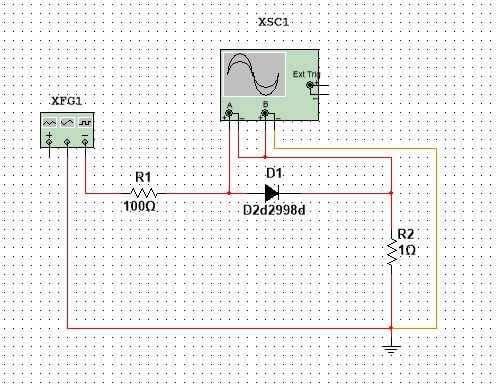
\includegraphics[width=0.6\textwidth]{img/15.jpg}
	\end{figure}
	\item Настроил генератор
	\begin{figure}[H]
		\centering
		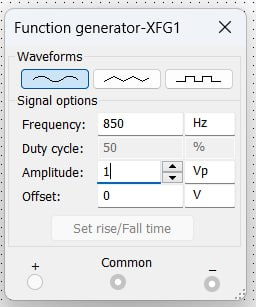
\includegraphics[width=0.4\textwidth]{img/16.jpg}
	\end{figure}
	\newpage
	\item Настроил осиллограф и получил его ВАХ на экране
	\begin{figure}[H]
		\centering
		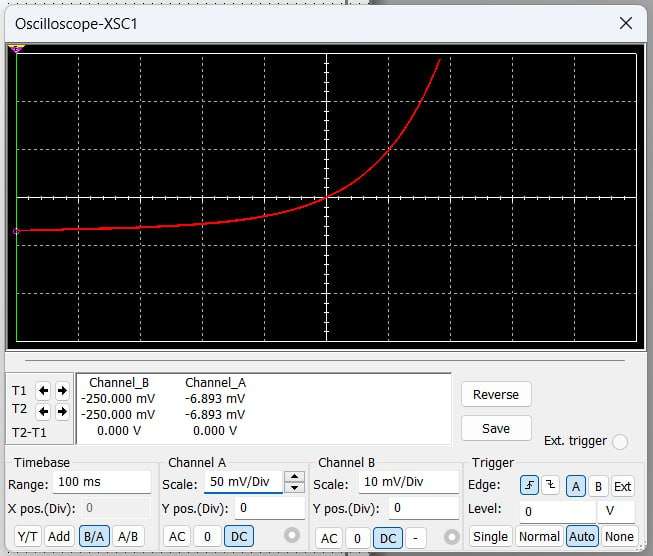
\includegraphics[width=0.65\textwidth]{img/17.jpg}
	\end{figure}
	\item Получил следующих график в \texttt{Grapher View}
	\begin{figure}[H]
		\centering
		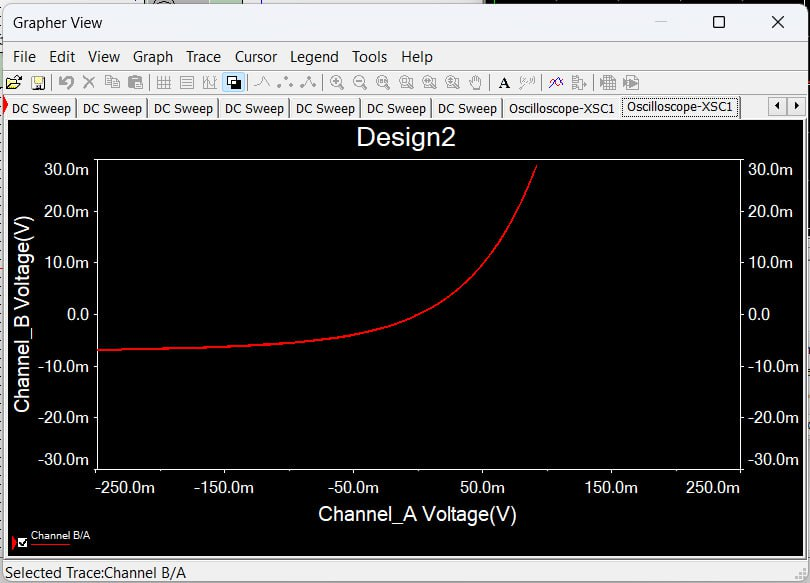
\includegraphics[width=0.65\textwidth]{img/18.jpg}
	\end{figure}
	\newpage
	\item Сохраню полученные данные в текстовом файле и открыл его в \textit{MathCAD}
	\begin{figure}[H]
		\centering
		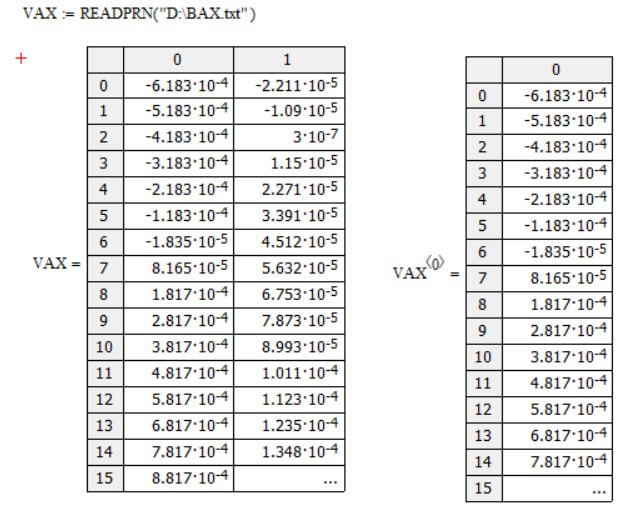
\includegraphics[width=0.6\textwidth]{img/19.jpg}
	\end{figure}
	\item Построил ВАХ
	\begin{figure}[H]
		\centering
		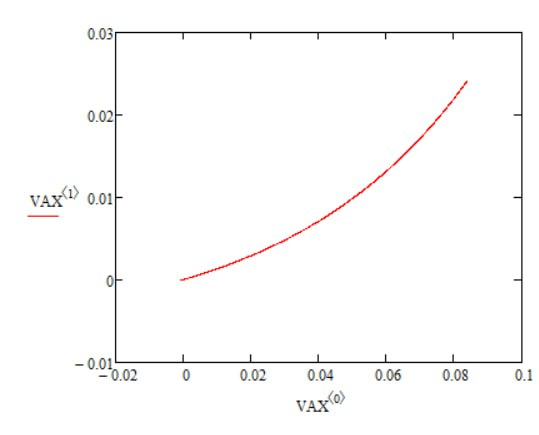
\includegraphics[width=0.6\textwidth]{img/20.jpg}
	\end{figure}
	\newpage
	\item Нашел теоретические характеристики диода, выбрав 3 произвольные точки на
	графике
	\begin{figure}[H]
		\centering
		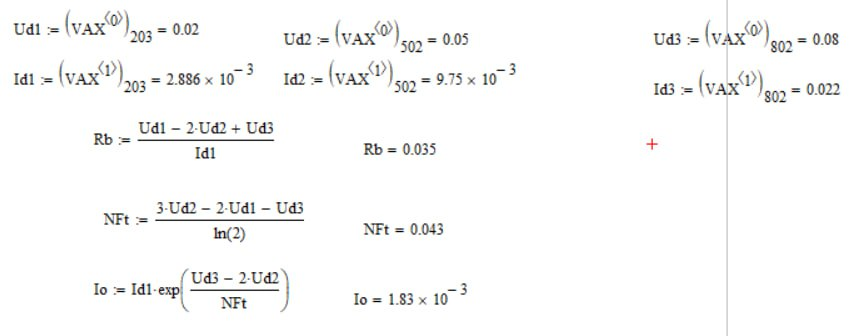
\includegraphics[width=0.6\textwidth]{img/21.jpg}
	\end{figure}
	\item Взял четвертую точку и рассчитал характеристики диода методом \textit{Given
	Minerr}
	\begin{figure}[H]
		\centering
		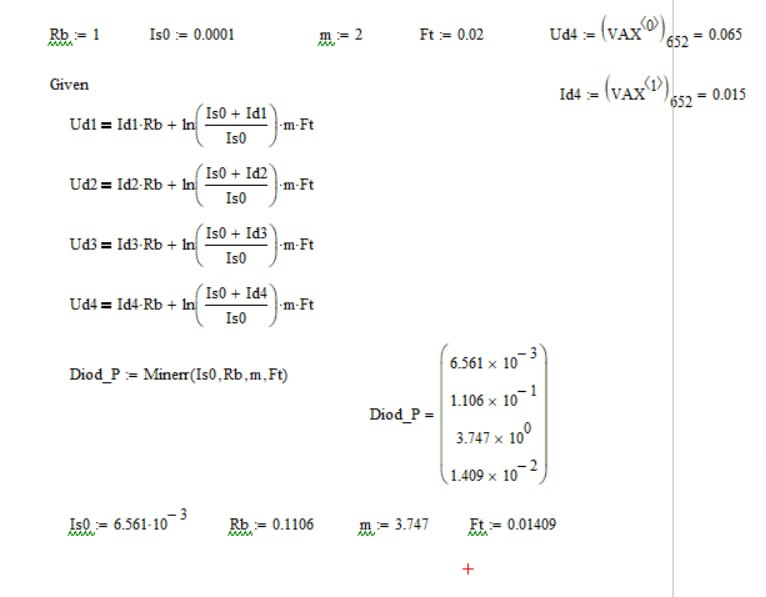
\includegraphics[width=0.55\textwidth]{img/22.jpg}
	\end{figure}
	\newpage
	\item Выполнил сравнение практических и теоретических данных, в моем случае
	максимальное значение силы тока не превышает 0.03
	\begin{figure}[H]
		\centering
		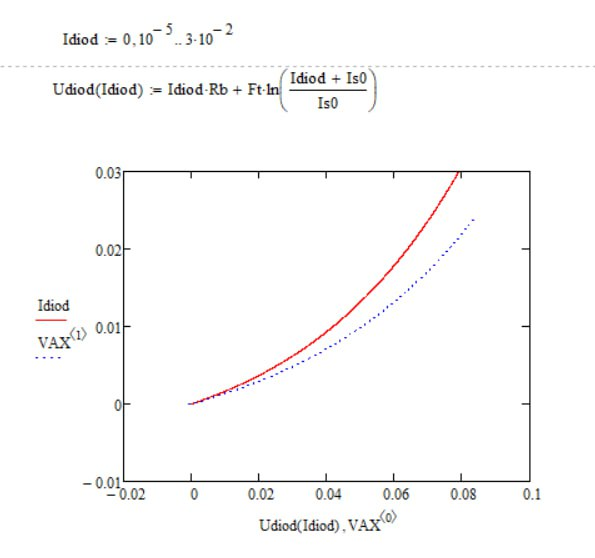
\includegraphics[width=0.6\textwidth]{img/23.jpg}
	\end{figure}
\end{enumerate}
